
\chapter{研究介紹}
\label{章:研究介紹}

\section{翻譯架構}
\label{節:翻譯架構}
因為閩南語目前閣無剖析的程式,本論文用的是斷詞翻譯\footnote{請看\ref{小節:斷詞翻譯}小節的紹介}

\section{語料形式選擇}
\label{節:語料形式選擇}
咱若共\ref{節:改變語料格式}節佮\ref{節:未知詞另外翻譯}節的方法合做伙,效果上好的是斷詞組對斷詞組,毋過斷詞組需要用剖析器去揣結構樹,閣來定規則決定詞佮詞啥物時陣愛敆做伙變詞組,這就是另外一門學問矣。目前閩南語閣無這資源,自然賰「華語斷詞-閩南語斷字」佮「華語斷詞-閩南語斷詞」上好,準若有好的斷詞工具,閩南語斷詞模型應該愛比閩南語斷字模型閣較好,雖然佇這擺實驗斷詞模型顛倒較\ji{⿰禾黑},毋過為著未來閩南語的斷詞研究方便比較,後壁的實驗模型攏是用「華語斷詞-閩南語斷詞」。
%------------------
加入新聞語料庫、教育部辭典佮數位典藏了後,按呢華臺平行語料有98814句\footnote{新聞語料庫64121句,教育部辭典34693句},會當訓練語言模型的閩南語有\footnote{新聞語料庫64121句,教育部辭典例句34693句、附錄句388句,數位典藏416343句},這个數量對照別種語言語料庫的數量也是小可嫌少。
佇這个網路的時代,收集語料上緊的方法就是去網路面頂掠。看圖XX,先共閩南語專門的字詞擲去搜尋引擊\footnote{親像Google、Bing},閣照揣著的網頁去掠相關的閩南語。
閩南語的網頁內底除了閩南語以外,有可能閣濫一部份的華語,為著莫予華語語料影響著閩南語模型,所以愛想辦法共臺華兩種語言分開。分開了後

%圖:關鍵詞 引擊 網址 掠網頁 網頁html 轉文字 一句一句的語料 判斷語言 閩南語/華語 對齊

\begin{figure}
\centerline{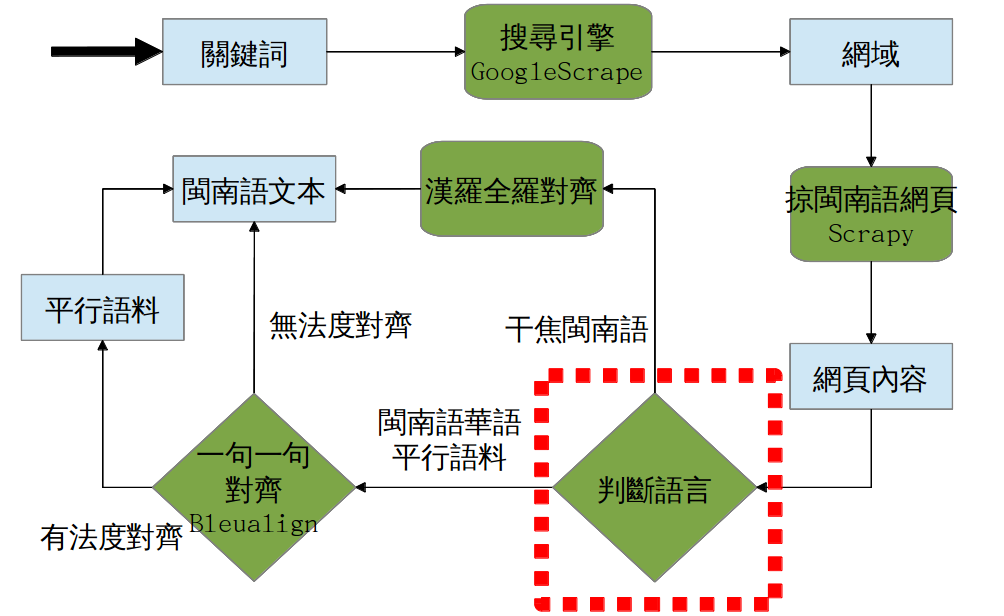
\includegraphics[keepaspectratio]{圖/網路語料庫結構}}
\caption{網路語料庫}
\label{圖:網路語料庫結構}
\end{figure}


\section{未知詞問題}
\label{節:未知詞問題}
系統結構會當看圖,語言模型用Witten-Bell加discounting的算法,翻譯模型用預設的參數。

訓練語料用新聞語料庫頭前2300篇新聞,攏總57167句,試驗語料用上尾267篇新聞,攏總6954句。按呢無調整語料,直接照伊的斷詞組落去訓練,共結果佮答案一句內底拆做一字一字,用\ref{節:評分方式}的BLEU去算分數,得著70.67分。

詳細看分數歹的原因,是因為傷濟詞組佇訓練語料無出現過,親像提原本試驗語料的華語句「陸續 開放 一百五十項 的 規費」去翻譯,得著「liok8-siok8 khai1-hong3 一百五十項 e5 規費」 ,「一百五十項」無翻譯出來,是因為訓練語料內底無出現過這个詞組,對訓練語料來講,「一百五十項」就是一个未知詞組。但是訓練語料內底有「兩項」佮「一百五十位」的華語詞組,煞無法度提來用。

為著予翻譯的結果閣較好,按算用兩種方式來加強未知詞的處理,頭一个是改變翻譯的單位,共原本斷詞組的語料改做斷詞抑是斷字,寫佇\ref{節:改變語料格式}節。第二个方法仝款照斷詞組翻譯,若拄著未知詞,針對未知詞專工處理,會當看\ref{節:未知詞另外翻譯}節。
